\chapter{Конструкторская часть}
В этом разделе будут представлены схемы алгоритмов для вычисления расстояний Левенштейна и Дамерау~---~Левенштейна.

\section{Разработка алгоритмов}

На рисунке~\ref{fig:rl} приведена схема рекурсивного алгоритма нахождения расстояния Левенштейна.

\begin{figure}[H]
	\centering
	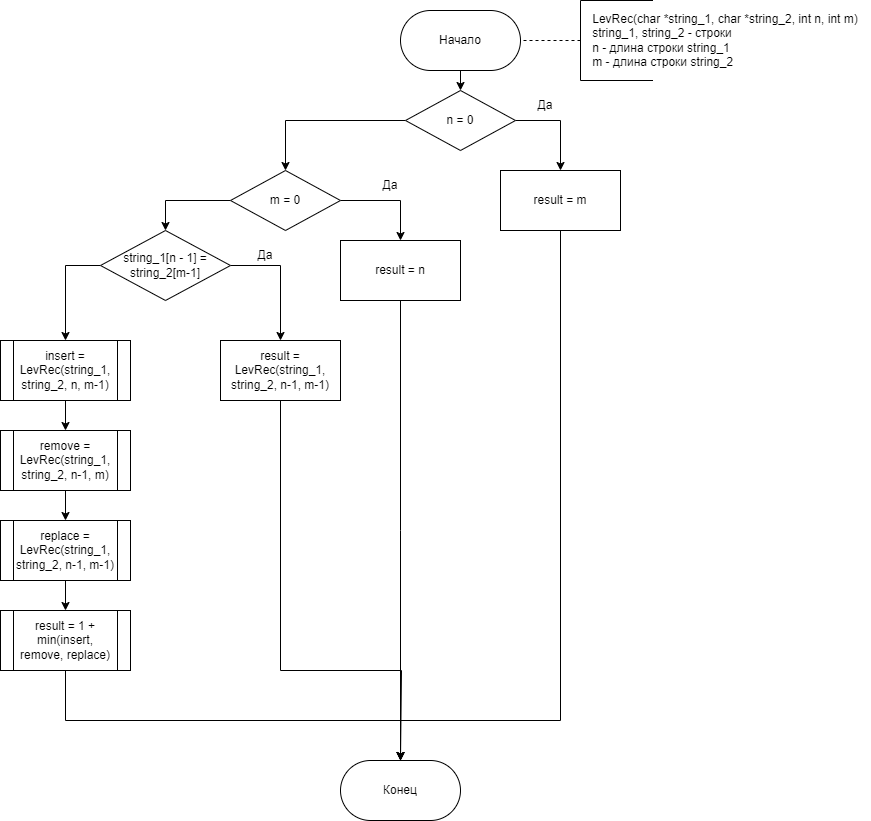
\includegraphics[height=0.65\textheight, page=1]{inc/img/AlgoSchems-LevRec.drawio.png}
	\caption{Cхема рекурсивного алгоритма нахождения расстояния Левенштейна.}
	\label{fig:rl}
\end{figure}

\newpage

На рисунке~\ref{fig:rlc} приведена схема рекурсивного алгоритма нахождения расстояния Левенштейна с кэшем.

\begin{figure}[H]
	\centering
	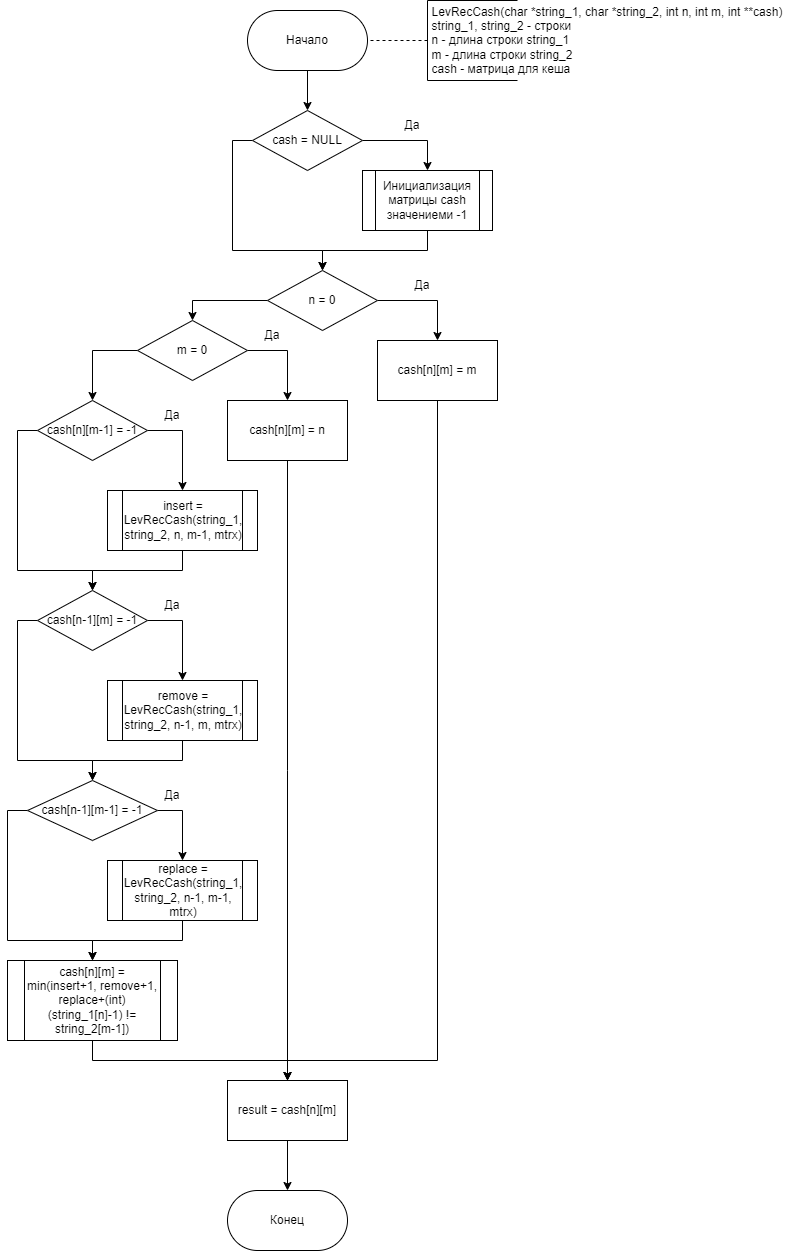
\includegraphics[height=0.85\textheight, page=1]{inc/img/AlgoSchems-LevRecCash.drawio.png}
	\caption{Cхема нерекурсивного алгоритма нахождения расстояния Левенштейна с кэшем.}
	\label{fig:rlc}
\end{figure}

\newpage

На рисунке~\ref{fig:nrl} приведена схема нерекурсивного алгоритма нахождения расстояния Левенштейна.

\begin{figure}[H]
	\centering
	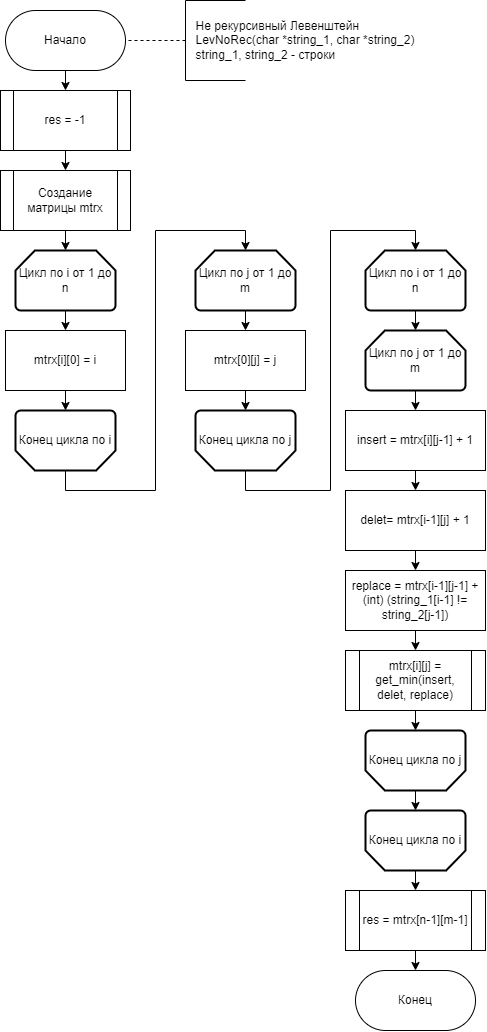
\includegraphics[height=0.85\textheight, page=1]{inc/img/AlgoSchems-LevNoRec.drawio.png}
	\caption{Cхема нерекурсивного алгоритма нахождения расстояния Левенштейна.}
	\label{fig:nrl}
\end{figure}

\newpage

На рисунке~\ref{fig:dl} приведена схема нерекурсивного алгоритма нахождения расстояния Дамерау~---~Левенштейна.

\begin{figure}[H]
	\centering
	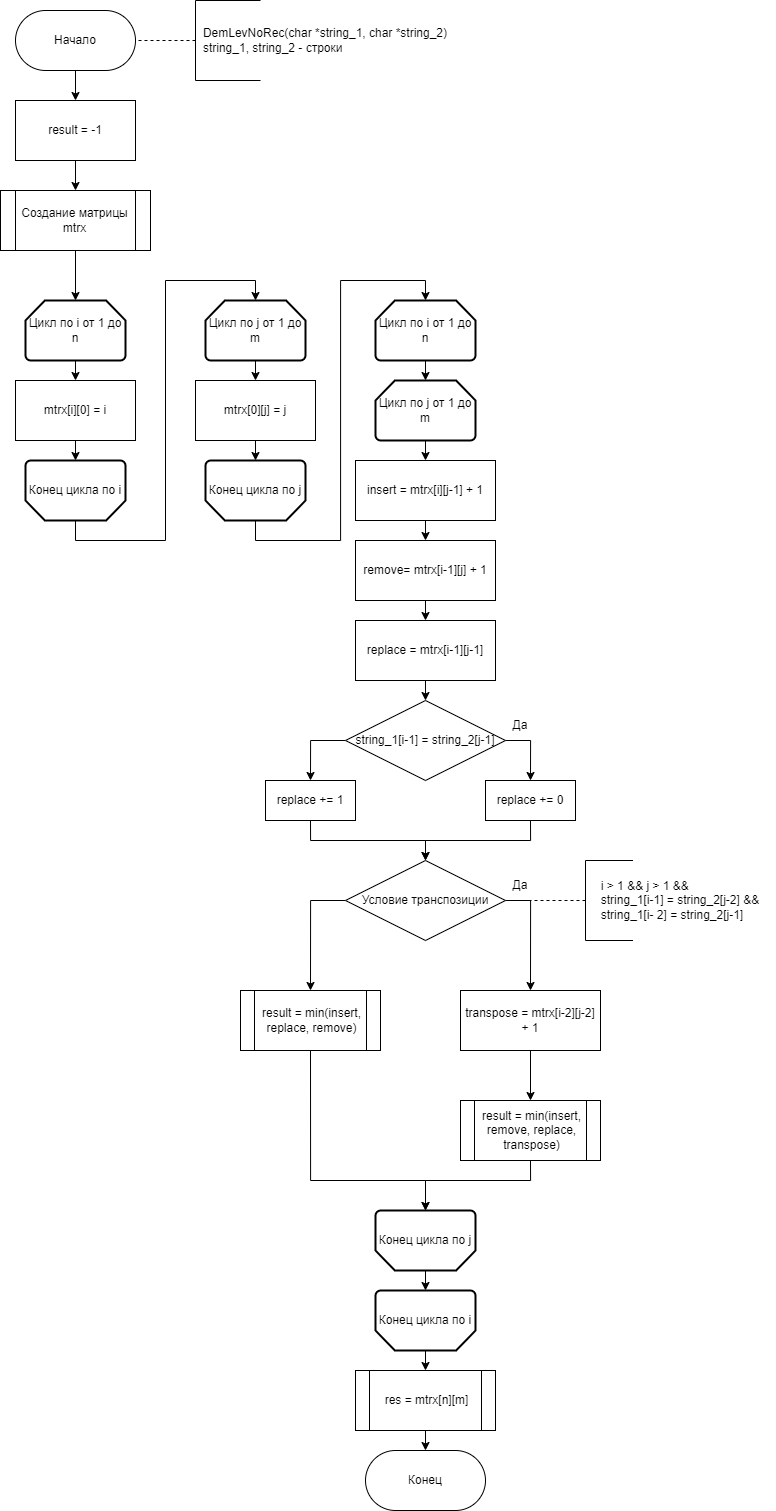
\includegraphics[height=0.85\textheight, page=1]{inc/img/AlgoSchems-DemLevNoRec.drawio.png}
	\caption{Cхема нерекурсивного алгоритма нахождения расстояния Дамерау~---~Левенштейна}
	\label{fig:dl}
\end{figure}

\newpage

\section*{Вывод}

В данном разделе были разработаны схемы необходимых алгоритмов, опираясь на данные, представленные в аналитической части.
